\documentclass[mathserif,spanish]{beamer}


\mode<presentation> {

% Algunos estilos para la presentación pueden elegir, el que mas le guste

%\usetheme{default}
%\usetheme{AnnArbor}
%\usetheme{Antibes}
%\usetheme{Bergen}
%\usetheme{Berkeley}
%\usetheme{Berlin}
%\usetheme{Boadilla}
%\usetheme{CambridgeUS}
%\usetheme{Copenhagen}
%\usetheme{Darmstadt}
%\usetheme{Dresden}
%\usetheme{Frankfurt}
%\usetheme{Goettingen}
%\usetheme{Hannover}
%\usetheme{Ilmenau}
%\usetheme{JuanLesPins}
%\usetheme{Luebeck}
%\usetheme{Madrid}
%\usetheme{Malmoe}
%\usetheme{Marburg}
%\usetheme{Montpellier}
%\usetheme{PaloAlto}
%\usetheme{Pittsburgh}
%\usetheme{Rochester}
%\usetheme{Singapore}
%\usetheme{Szeged}
\usetheme{Warsaw}

% As well as themes, the Beamer class has a number of color themes
% for any slide theme. Uncomment each of these in turn to see how it
% changes the colors of your current slide theme.

%\usecolortheme{albatross}
%\usecolortheme{beaver}
%\usecolortheme{beetle}
%\usecolortheme{crane}
%\usecolortheme{dolphin}
%\usecolortheme{dove}
%\usecolortheme{fly}
%\usecolortheme{lily}
%\usecolortheme{orchid}
%\usecolortheme{rose}
%\usecolortheme{seagull}
%\usecolortheme{seahorse}
%\usecolortheme{whale}
%\usecolortheme{wolverine}

%\setbeamertemplate{footline} % To remove the footer line in all slides uncomment this line
\setbeamertemplate{footline}[page number] % To replace the footer line in all slides with a simple slide count uncomment this line

%\setbeamertemplate{navigation symbols}{} % To remove the navigation symbols from the bottom of all slides uncomment this line
}

\usepackage{graphicx}
\usepackage{booktabs} 
\usefonttheme{professionalfonts}
\usepackage{beamerthemesplit}
\usepackage[justification=centering]{caption}
\setbeamertemplate{caption}[numbered]
\usepackage{ragged2e}
\justifying
\usepackage{hyperref}
\usepackage{chngcntr}
\usepackage[utf8]{inputenc} 
\usepackage[spanish]{babel}

% Titulo principal del portada de la diapositiva

\title[Resultados del laboratorio XX]{Resultados del laboratorio 02} % Titulo de la presetación
\subtitle{Equipo A} % Grupo asignado
\author[F.Chacón \and J.Quirós \and A.Volta]{F.Chacón \and J.Quirós \and G.Araya} % Autores
\institute[Instituto Tecnológico de Costa Rica]{
Instituto Tecnológico de Costa Rica\\
Escuela de Ingeniería Electrónica \\
Identificación y control del péndulo amortiguado a hélice (PAMH)} % 
\date{\today}

% Iniciamos con la presentación
\begin{document}

    \begin{frame}[plain]
        \begin{center}
            
\includegraphics [height=3cm,width=6cm]{TEC}    % Imagen del TEC
        \end{center}
        \titlepage
    \end{frame}

    \begin{frame}{Contenidos} % Se muestran los contenidos que serán abordados en la presentación
        \tableofcontents 
    \end{frame}

% Slides de la presentación

\section{Introducción}          % Sección de introducción

\subsection{Resumen}            % Subsección de resumen
    \begin{frame}{Resumen}
        Mediante la herramienta Pascal se procederá a la recopilación de los datos generados por un motor de CD, luego de activarlo con pulsos de tipo escalón, dichos pulsos con diferentes duraciones con el fin de obtener un modelo matemático empírico que describa su comportamiento, luego con las herramientas para análisis de control automático que dispone "Matlab" se procederá a diseñar un controlador PID. Luego a un modelo matemático propuesto,se le procederá por medio de herramientas de software a generar un sistema de control PID n el fin  el fin de controlar su estabilidad, el cual pasara un proceso de sintonización.  el se procede a implementarlo en Pascal, por medio del cual se verifica su funcional.   \end{frame}

\subsection{Objetivos Generales}
    \begin{frame}{Objetivos Generales}
        \begin{itemize}
            \item Obtener el Modelo matemático empírico con datos de campo de una planta "Motor CD".
            \item Con base a un modelo matemático proceder a analizar, sintonizar e implementar un sistema de control PID.
        \end{itemize}
    \end{frame} % Subsección de objetivos generales

\subsection{Objetivos Específicos}
    \begin{frame}{Objetivos Específicos}
        \begin{itemize}
            \item Obtener datos por medio de la aplicación Pascal
            \item Obtener el Modelo empírico de la velocidad de un Motor CD
            \item Procesamiento de Datos experimentales
            \item Diseñar un regulador PID para modelo matemático 
            \item Calibrar o sintonizar implementación de modelo
            \item Probar el diseño por medio de la aplicación Pascal
        \end{itemize}
    \end{frame}   % Subsección de objetivos específicos

\section{Metodología de medición}   % Sección de metodología
    \subsection{Obtener el Modelo empírico de la velocidad de un Motor CD}
        \begin{frame}{Metodología}
             \item 
           por medio de         
\begin{figure}[!h]
\centering
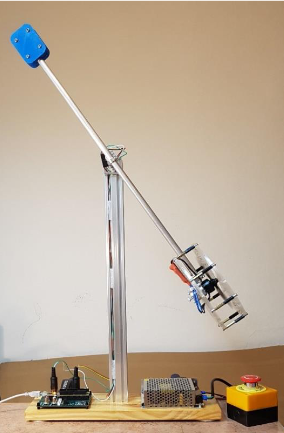
\includegraphics[width=0.35\textwidth]{L02img01.png}
\caption{Fotografía del sistema de péndulo amortiguado a hélice}
\label{fig:comp_cd}
\end{figure}
        
       \end{frame}


    \subsection{Obtener datos por medio de la aplicación Pascal}
        \begin{frame}{Metodología}
              \item 
                 
        \begin{figure}[!h]
\centering
\includegraphics[width=0.45\textwidth]{Img04.png}
\caption{Datos en formato .csv}
\label{fig:rlocus1}
\end{figure}
        
      \end{frame}


    \subsection{Procesamiento de Datos experimentales}
        \begin{frame}{Metodología}
             \item 
                 
        \begin{figure}[!h]
\centering
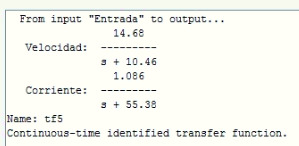
\includegraphics[width=0.45\textwidth]{img02.jpeg}

\label{fig:rlocus1}
\end{figure}

        \begin{figure}[!h]
\centering
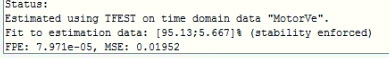
\includegraphics[width=0.45\textwidth]{img01.jpeg}
\caption{Función de transferencia}
\label{fig:rlocus1}
\end{figure}
        
            \end{frame}


    \subsection{Diseñar un regulador PID en sisotool}
        \begin{frame}{Metodología}
               \item 
                 
        \begin{figure}[!h]
\centering
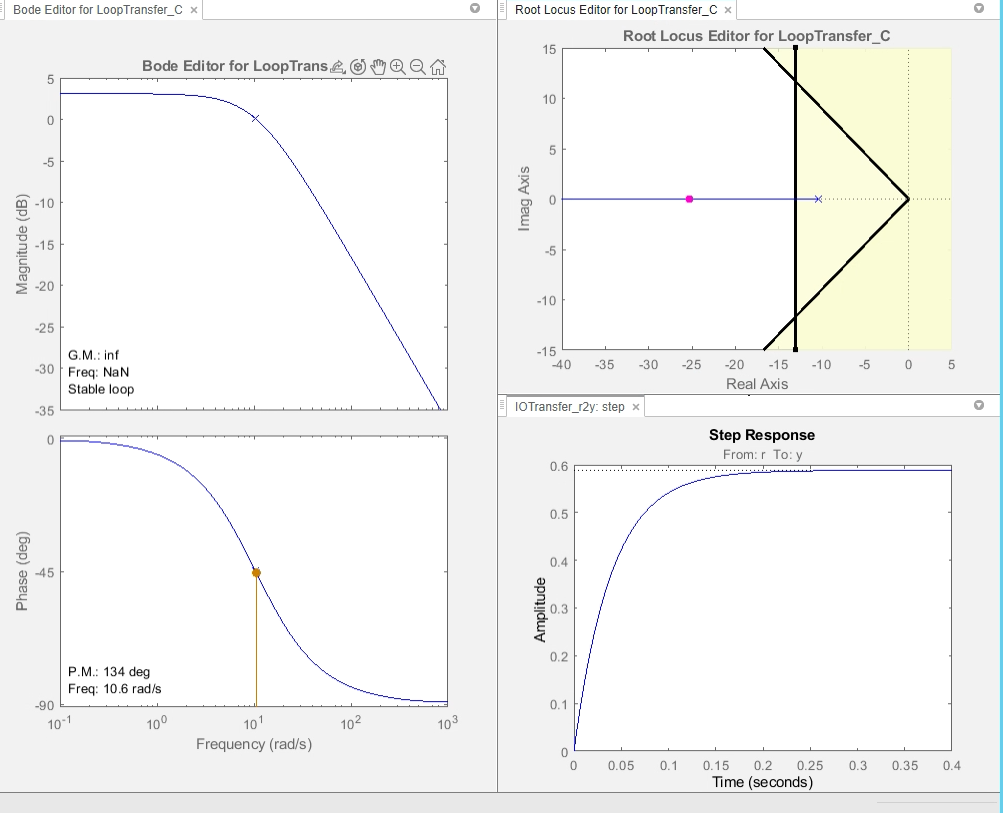
\includegraphics[width=0.45\textwidth]{img05.png}
\caption{Respuesta del modelo sin control}
\label{fig:rlocus1}
\end{figure}
        
        \end{frame}
    
        \begin{frame}{Metodología}
               \item 
                 
        \begin{figure}[!h]
\centering
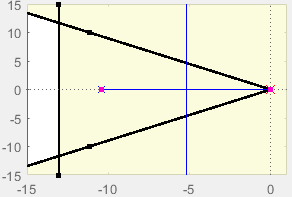
\includegraphics[width=0.45\textwidth]{rlocuspolo.png}
\caption{Lugar de las raíces con polo s=0}
\label{fig:rlocusp}
\end{figure}
\end{frame}

        \begin{frame}{Metodología}
\begin{figure}[!h]
\centering
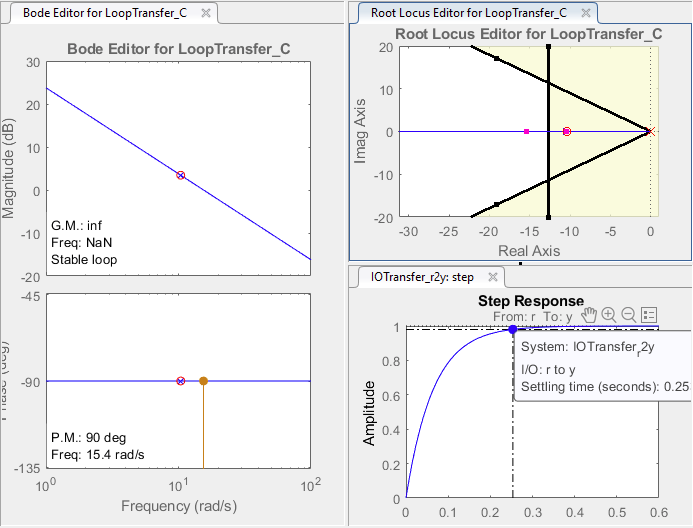
\includegraphics[width=0.55\textwidth]{final.png}
\caption{Respuesta del modelo con PI}
\label{fig:rfinal}
\end{figure}
        
        \end{frame}

    
        \begin{frame}{Metodología}
               \item 
                 
        \begin{figure}[!h]
\centering
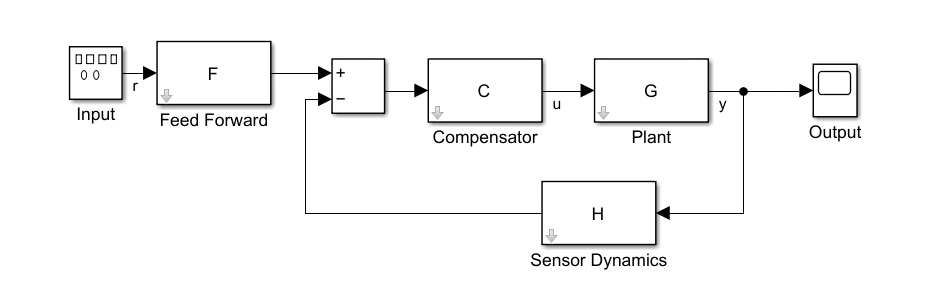
\includegraphics[width=0.45\textwidth]{img06.png}
\caption{Modelo de bloque  }
\label{fig:rlocus1}
\end{figure}
        
       \end{frame}










\section{Análisis de Resultados}   % Sección de metodologí
    \subsection{Análisis de Resultados}
         \begin{frame}{Análisis de Resultados}
         \begin{figure}[!h]
\centering
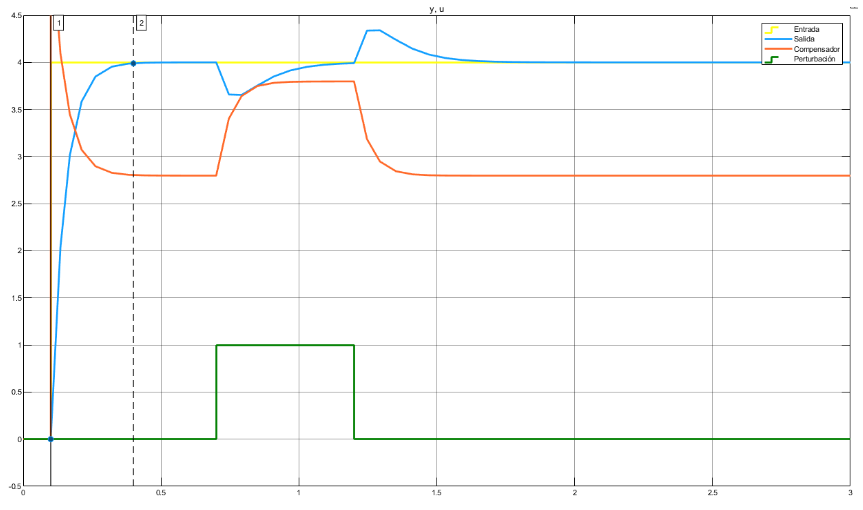
\includegraphics[width=0.6\textwidth]{simu_matl.png}
\caption{Simulación en matlab del sistema PI con perturbaciones}
\label{fig:simu_mat}
\end{figure}

        \end{frame}
        \begin{frame}{Análisis de resultados}

                 \begin{figure}[!h]
\centering
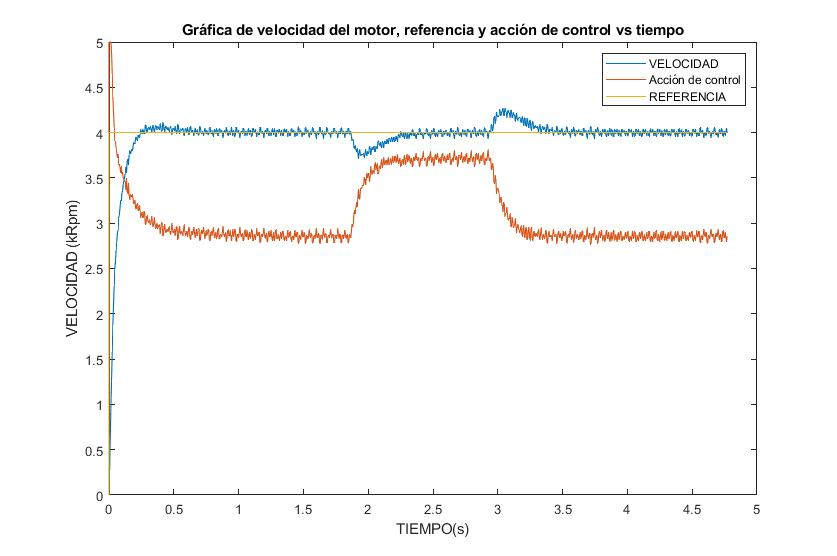
\includegraphics[width=0.7\textwidth]{RESULTADOS_MOTOR_CD.jpg}
\caption{Respuesta del sistema controlado a nivel experimental}
\label{fig:tabla_re}
\end{figure}
            
        \end{frame}

        \begin{frame}{Análisis de resultados}

                 \begin{figure}[!h]
\centering
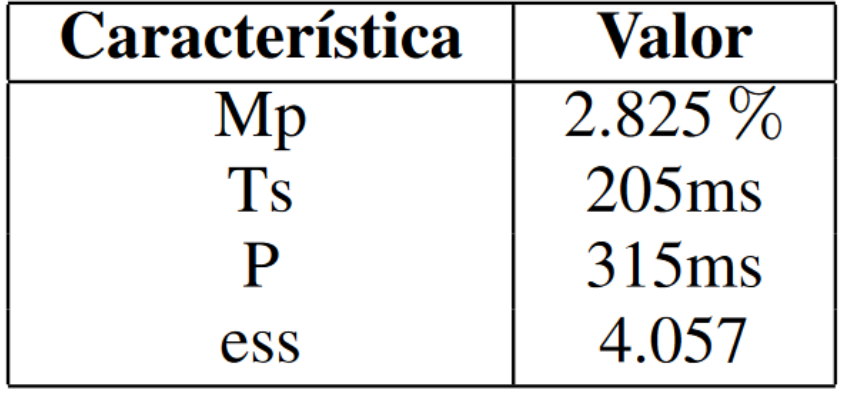
\includegraphics[width=0.45\textwidth]{tabla_result.png}
\caption{Parámetros obtenidos de resultados experimentales}
\label{fig:tabla_re}
\end{figure}
            
        \end{frame}
\section{Conclusiones}              % Sección de conclusiones
    \subsection{Conclusiones}       % Subsección de conclusiones
        \begin{frame}{Conclusiones}
            Se representó el modelo empírico del motor CD demostrado en la ecuación inicial, este obtuvo un porcentaje de ajuste equivalente a 95.13\% relacionado al control de velocidad.

\newline

Se diseñó un regulador electrónico proporcional e integral mediante ubicación de polos, esto permitió mejorar los resultados de la función de transferencia original, se ajustó un sobreimpulso menor al 3\% con un tiempo de estabilización menor a 300ms, además el error de estado estacionario se ubicó en cero
        \end{frame}
    \subsection{Conclusiones}       % Subsección de conclusiones
        \begin{frame}{Conclusiones}
        
        La simulación del sistema controlado permitió demostrar cuantitativamente los resultados de la implementación simulada mediante el control proporcional e integral, de esta manera se comprobó el ajuste correcto de los parámetros con base a los requisitos para la prueba experimental.

La comprobación experimental del controlador PI dio como resultado un porcentaje de sobreimpulso de 2.825\% y un tiempo de estabilización de 205ms, estos parámetros antes mencionados cumplen con los requisitos del laboratorio. El error de estado estacionario es de 4.057 y el tiempo de estabilización ante perturbaciones de 315ms, en este caso ambos parámetros no cumplen con los requisitos de laboratorio al momento de realizar el experimento.
\end{frame}
    \section{Recomendaciones}    % Subsección de recomendaciones
        \begin{frame}{Recomendaciones}
        \begin{itemize}
            \item Tiempo
            \item Modelo
            \item Ruido y componentes externos
            \item Aumentar la velocidad sin pasar de 3$\%$ de sobre impulso 
        \end{itemize}
            %Se le pide al menos, que expongan algunas limitaciones que tuvieron a la hora de realizar el laboratorio y expongan alguna recomendación para mejoras a futuro del laboratorio.
        \end{frame}
%------------------------------------------------


\end{document}